\section{Study protocol}

\subsection{Overview of the study}
\label{subsection:overview-study}

\subsubsection{General procedure}
This study considers a 2x2 split-plot design~\cite{lazar-hci-2017} to quantify the behavioral and performance cost of digital newspaper documents under \CVAS. The objective is to understand how these individuals (readers with normal vision on small displays and readers with low vision even in larger displays) consume these digital documents. Approval for this research was granted by Inria’s Operational Committee for the Assessment of Legal and Ethical Risks.

To create controlled yet realistic reading conditions, text-only newspaper pages were considered, each composed of multiple blocks containing one headline and a body text (\secref{sec:newspaperpages}). This approach provides two key advantages:
\begin{itemize}
    \item Controlled entry points: Headlines serve as the sole entry points, ensuring that participants’ reading path relies on a textual structure that can be controlled and standardized. This also allow to track the sequence in which participants access articles through aloud reading, a practical alternative to eye-tracking, which is difficult to implement with participants \LV.
    \item Reduced cross-trial variability: By avoiding graphical elements (e.g., advertisements, photographs, or diagrams), which are harder to standardize, we minimize potential confounds across trials and conditions, ensuring comparability of reading behavior data.
\end{itemize}

It is important to note that the use of text-only newspaper pages does not compromise the ecological validity of the study. The primary focus is on the reading behavior and navigation strategies of participants under \CVAS, which are expected to be consistent across both text-only and multimodal newspaper pages. The controlled environment allows for a more precise assessment of the impact of layout and magnification conditions on reading performance and cognitive load.


The experiment consisted of two tasks designed as controlled proxies of real-world newspaper consumption strategies, allowing for systematic observation and quantification of reading behavior:
\begin{itemize}
\item {\bf Task 1 (structural orientation):  read all headlines.} \\This task emulates the initial scanning phase of newspaper consumption. Participants read aloud all headlines on a page, as fast but intelligibly as possible, in any order they wished. Reading aloud allow to unambiguously capture the order in which headlines were read, and is both a well-established method in reading research~\cite{wang_understanding_2023, wang_gazeprompt_2024} and clinical assessments (e.g., MNREAD). This task addressed \hypperformance and \hyppath. There was no time limit. Participants decided themselves when they had finished, even if some headlines were missed.

\item {\bf Task 2 (targeted information retrieval): find a target headline.} \\ This task tests the user's mental representation of the page and their ability to retrieve specific information. Participants were asked to locate a specific headline containing a given keyword, to probe their mental representation of page structure. This task tested the hypothesis \hypfindingperformance. To examine \hypfindingpositions,  the page was divided into three vertical zones (top, middle, bottom) and selected two targets per zone. The order is random for each participant, and the zone division is not disclosed. Each search trial was limited to one minute.
\end{itemize}


Both tasks were performed under \condonenot and \condtwonot. A critical design feature of this protocol is to ensure that participants had to rely on \panzoom in \condonenot but could comfortably read headlines in \condtwonot. To achieve this,  each participant’s Critical Print Size (CPS)~\cite{legge2006} was determined, defined as the smallest print size allowing readers to maintain maximum reading speed, and expressed in logMAR units (logarithm of the Minimum Angle of Resolution), which quantify text size in terms of visual angle rather than physical dimensions, which is crucial because it jointly depends on both print size in millimeters and viewing distance. Headlines in \condonenot are below each participant’s CPS, forcing gesture-based magnification, while in \condtwonot they were manually set above CPS, enabling comfortable direct reading. 

As a note, integrating eye-tracking to capture complementary gaze data was considered. However, it was discarded  due to specific challenges for this study. First, in this context, fixations mix cognitive inspection with smooth pursuit driven by viewport motion, and gaze positions must be continuously remapped to a moving document coordinate system, which limits interpretability~\cite{heo_reading_2024, jacob_eye_2003, valsecchi_saccadic_2013}. Second, there is a limitation to obtain a precise calibration with participants with low vision, since precise calibration requires an intact fovea which is usually not the case~\cite{wang_understanding_2023, heo_reading_2024}. Although technically feasible thanks to workarounds that mitigate the underlying issues, these constraints would have reduced the validity of the resulting metrics for the desired goal, which was to characterize reading strategies at a macroscopic level, not fine-grained oculomotor behavior. 


Following these principles, the study protocol unfolded in five steps, summarized in \figref{fig:protocole-overview}. 
\begin{enumerate}
    \item Participants first completed a short questionnaire about gender, age group, and reading habits (general and news-specific). 
     \item A standard MNREAD test~\cite{legge2006} to estimate each participant’s Critical Print Size (CPS) was applied. 
    \item Based on the CPS, the proposed protocol define how the two conditions would be instantiated (see \secref{sec:condition-definition}), including the choice of device (small-screen phone for participants with normal or corrected-to-normal vision, large-screen tablet for participants with low vision) and the viewing distance to be maintained during the experiment.
    \item After a detailed explanation of the protocol, participants proceeded to the main experiment. Each block corresponded to one condition, with the order counterbalanced across participants.
    \begin{itemize}
        \item To familiarize themselves with the tasks, participants first completed as many practice trials as needed. We used three fixed layouts (same order for everyone), and cycled through them if more than three trials were required. In practice, one or two trials were sufficient. 
        \item Participants then completed $M$ test trials per condition. Number of trials $M$ depending on the participant scenario (see \secref{sec:protocole-adjustements-nv} and \secref{sec:protocole-adjustements-lv}). Layouts were randomized, and content was randomly assigned to conditions (see \secref{sec:newspaperpages})
        \item After each block, perceived workload was measured using the NASA-TLX questionnaire~\cite{hart_nasa-task_2006}, using a 7-point likert scale.
    \end{itemize}
    \item Finally, participants indicated their overall preference between \condonenot and \condtwonot (or equal preference).
\end{enumerate}
\begin{figure}[htbp]
    \centering
    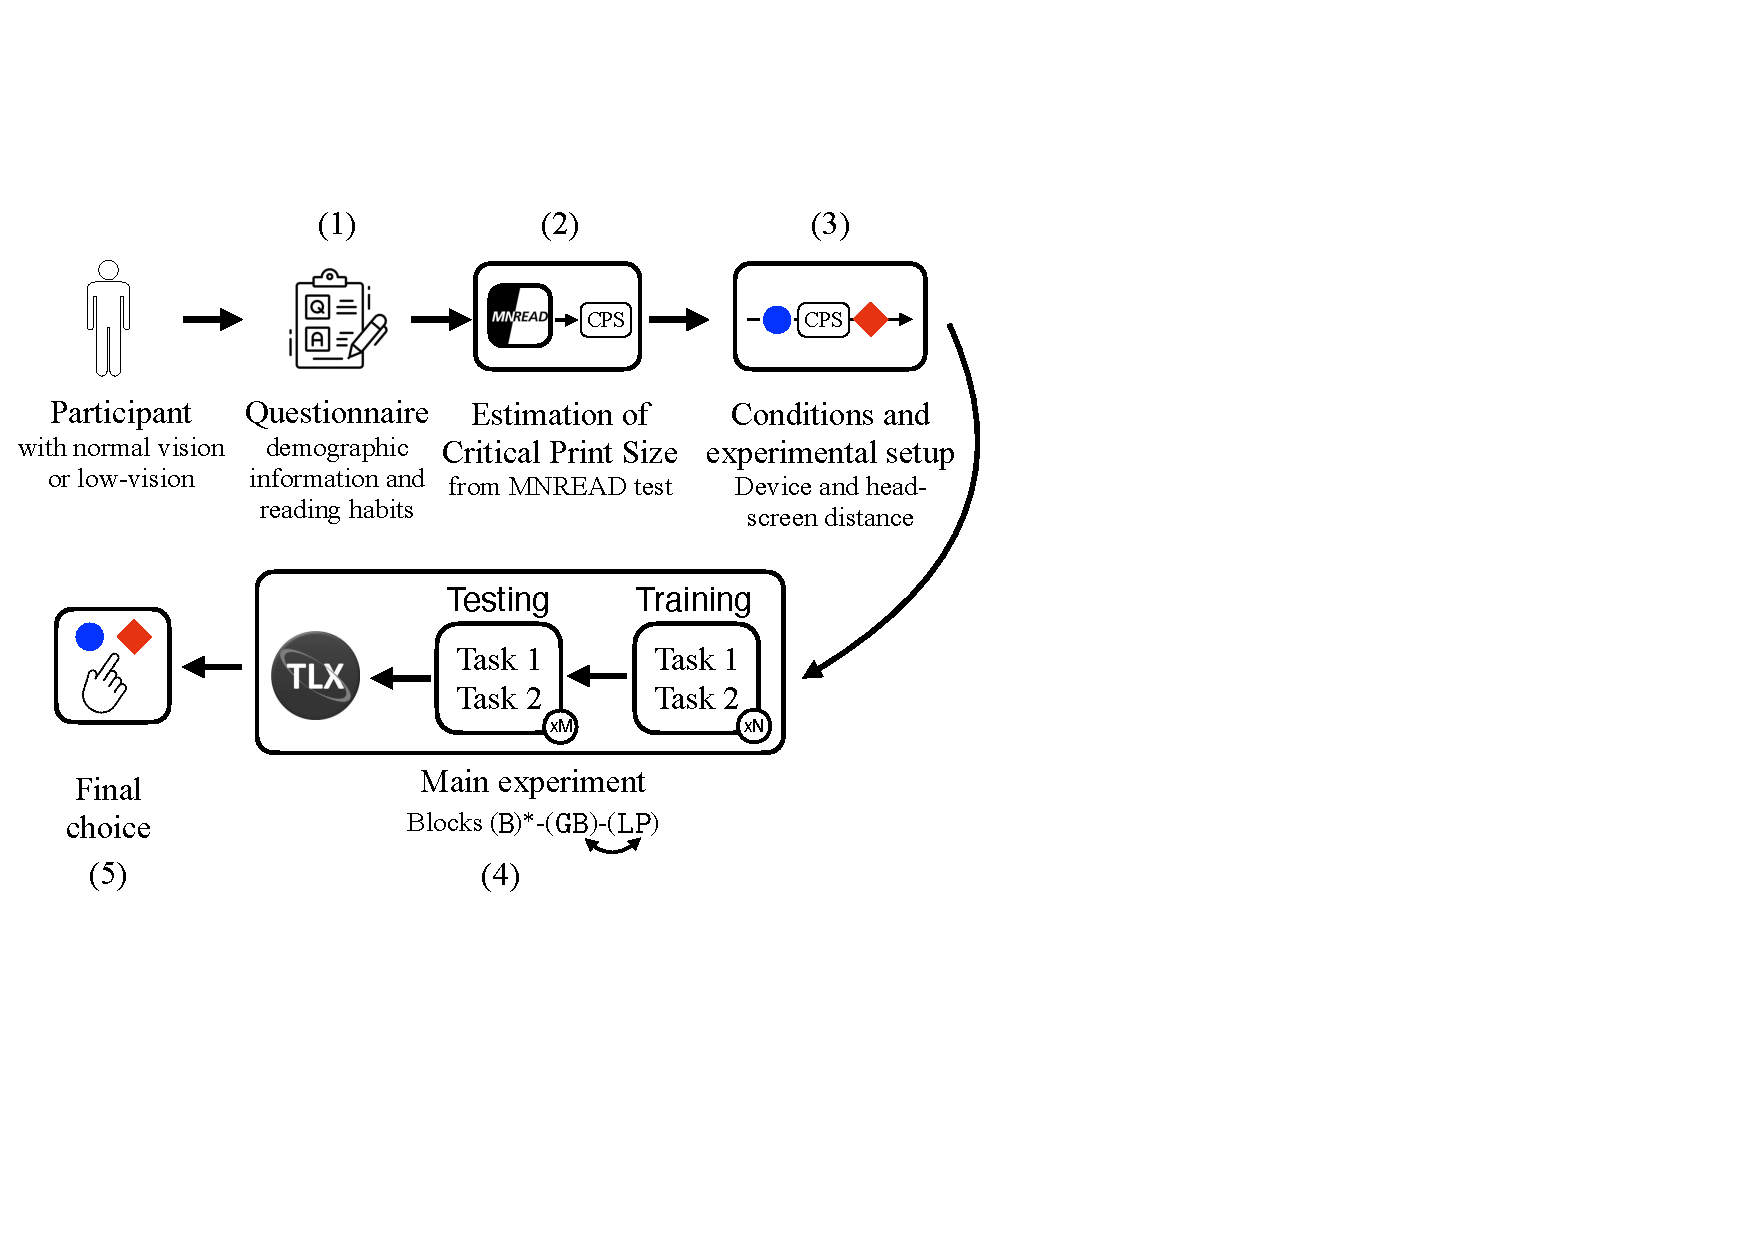
\includegraphics[width=\widthForOneImage]{img/protocole-overview.pdf}
    \caption{
    Overview of the study. This figure illustrates the workflow of our experimental protocol, organized into five main steps: (1) questionnaires, (2) estimation of Critical Print Size (CPS), (3) conditions and experimental setup, (4) the main experiment, and (5) a final preference choice. The main experiment consisted of successive blocks in the two conditions (\condonenot and \condtwonot).Some adjustments were made depending on the participant scenario. Each block included a training phase followed by test phases, where Tasks~1 and 2 were repeated across trials, and ended with the NASA-TLX questionnaire. The overall protocol lasted less than an hour, with the main experiment capped at 30 minutes to avoid excessive fatigue for participants with low vision.}
    \label{fig:protocole-overview}
\end{figure}

This protocol served as the common foundation of the study. However, some adjustments were necessary depending on the participant's scenario.
\subsubsection{Protocol adjustments: participants \NV}
\label{sec:protocole-adjustements-nv}
%%%%%%%%%%%%%%%%%%%%%%%%%%%%%%%%%%%%%%%%%%%%%%%%%%%%%%%%%%%%%%%%%%%%%%%%%%%%
First, after pilot studies to study participants' fatigue, number of trials ($M$) was tuned to $M=6$ testing trials for participants \NV.

Second,  an additional baseline condition (\condzeronot) was included and applied before \condonenot and \condtwonot, with the same trials configuration ($N$ for practice and $M=6$ for testing).

\condzeronot simulates the experience of reading a physical newspaper, corresponding to unconstrained reading. In this condition, the original edition was displayed on a large-screen tablet, with no magnification gestures, as headlines were already comfortably legible (approximately $0.3$ logMAR at 40\,cm). Note that this baseline was not feasible for participants \LV, since the original edition would remain unreadable without magnification, even on a tablet. Data from \condzeronot were used to define a natural reading path, coined reference paths in this thesis, and were compared to the paths observed in \condonenot and \condtwonot when testing hypothesis \hyppath. 


\subsubsection{Protocol adjustments: participants \LV}
\label{sec:protocole-adjustements-lv}
For participants \LV, pilot sessions revealed that 6 testing trials were overly demanding for this group: several participants suddenly experienced acute visual fatigue, making it impossible to continue and leading to early interruptions. As a consequence, this protocol design risked unbalancing the data, with many completing only a single condition. To address this, trials and blocks configuration was adjusted (changes in Fig~\ref{fig:protocole-overview} (4) and (5)):
\begin{itemize}
    \item Participants first completed two trials per condition, each followed by a NASA-TLX questionnaire, to ensure that subjective workload was captured before cumulative fatigue could bias responses.
    \item The order of layouts was randomized but kept identical across \condonenot and \condtwonot to support fair comparisons.
    \item To maximize usable data, participants continued with the remaining four trials per condition in an alternating sequence (one \condonenot, one \condtwonot, and so on). Sessions ended as soon as all trials were completed, the participant indicated they were too tired to continue, or the 30-minute time limit was reached.
    \item Finally, participants reported their overall preference between \condonenot and \condtwonot, or both equally. Because cumulative fatigue strongly influenced judgments, a comparative NASA-TLX was administered at the end of the session to balance condition evaluations.
\end{itemize} 

Having outlined the overall procedure, the following sections expand on its key components.



